\documentclass[11pt,a4paper]{article}
\usepackage[margin=1.2in]{geometry}
\usepackage{times}
\usepackage{graphics}
\usepackage{graphicx}
\usepackage{natbib}
\usepackage{durhampaper}
\usepackage{subfigure}
\usepackage{todonotes}
\usepackage{glossaries}
\usepackage{booktabs}
\usepackage[font=small,labelfont=bf, textfont=it]{caption}
% \usepackage{harvard}
\usepackage[moderate]{savetrees}
\usepackage{url}
\usepackage{amsmath}

\makeglossaries
\title{Facial Liveness Testing: an approach for the web}
\author{} % leave; your name goes into \student{}
\student{Ryan Collins}
\supervisor{Prof A. Krokhin}
\degree{MEng Computer Science}

\date{\today}




% Now the main body of the document.
\begin{document}

\maketitle
\begin{abstract}
% These instructions give you guidelines for preparing the final paper.  DO NOT change any settings, such as margins and font sizes.  Just use this as a template and modify the contents into your final paper.  Do not cite references in the abstract.
% However, with facial recognition comes face spoofing: methods to fool the algorithms into thinking one is someone different to who they are.
% The abstract must be a Structured Abstract with the headings {\bf Context/Background}, {\bf Aims}, {\bf Method}, {\bf Results}, and {\bf Conclusions}.  This section should not be longer than half of a page, and having no more than one or two sentences under each heading is advised.
\paragraph{Context}
    With password based authentication methods being subject to many attacks, facial recognition is an alternative, relying on biometrics rather than remembering an easily stolen string of characters.
    While secure facial recongition methods have been developed, spoofing is still a concern. Spoofing is where someone tries to pretend they are someone else to gain access.
    In order for facial recognition to become more prevalent on the web, facial liveness is needed. Facial liveness methods don't check identity, but aim to detect these impersonation methods.
    The next step towards secure facial recognition systems are facial liveness services, which provide an indication of liveness and can be integrated into applications, through APIs on the internet.
    This paper aims to understand which liveness tests are suitable for deploying in such a service, and explains next steps and architectures to the development of a facial liveness service for the modern web.

\paragraph{Aims}
    % This might belong more in the method.

    \begin{itemize}
        \item Verify the results of the proposed Whole-Image Quality Assessment (W-IQA) test.
        \item Assess the outcome of a new ResNet based classifier on classifying real/spoofed images.
        \item Design and implement a new 3D based liveness test, aimed to prevent mask attacks.
        % \item Determine the outcome of fusing the three above methods together, and how successful this is.
    \end{itemize}

\paragraph{Method}
   \begin{itemize}
        \item The W-IQA liveness test was implemented in Python to consider the image as a whole.
        \item A CNN based 2D liveness test was implemented in Python to classify facial structure.
        \item A 3D based liveness test to detect mask attacks was designed and implemented, and assessed based on practicality for the web.
   \end{itemize}
\paragraph{Results}
    \begin{itemize}
        \item W-IQA test performed well, yielding 87\% accuracy over the Replay-Attack test dataset.
        \item CNN based 2D test performed adequately, yielding 71\% accuracy over the Replay-Attack test dataset.
        \item The VoxNet based 3D liveness test performed poorly, and had various performance issues that means it's not currently practical to deploy.
    \end{itemize}
\paragraph{Conclusions}
    Overall, both the Whole Image Quality assessment and CNN based 2D test are metrics to include in a liveness-as-a-service system.  The W-IQA test individually yields
    impressive results, but the CNN based metric would perform well when working together with other metrics. The CNN based metric could be further improved by adjusting preprocessing,
    and using a deeper ResNet pretrained model. The VoxNet model has also shown that this method is a poor liveness test for the existing use case, due to high computational requirements.
    In addition, the speed at which queries can be answered shows that these can reasonably be used in a web system without extensive delays in processing, or without requiring any additional hardware (aside from a camera).
\end{abstract}

\begin{keywords}
Facial liveness, convolutional neural networks, image quality metrics, residual networks, anti-spoofing
\end{keywords}

\section{Introduction}
    % What is the project about?
    % Currently, username and password authentication is commonplace throughout the web. However, username and password
    % based authentication systems have a number of problems. Some common passwords can be broken using dictionary attacks,
    % especially if they consist partially or entirely of a word in a standard dictionary. Furthermore, the process of shoulder surfing is possible (watching out
    % for someone's password, and how they type it).
    Currently, username and password authentication is commonplace throughout the web. However, this method has serious security concerns, being easily broken through dictionary attacks,
    or shoulder surfing. Facial recognition authentication doesn't have either of these problems, but introduces the risk of stolen identity through face spoofing, more specifically expressed
    in a quotation from Adam Schwartz, a lawyer with the Electronic Frontier Foundation speaking to NPR: "We can change our bank account numbers, we can even change our names, but we cannot change our faces.
    And once the information is out there, it could be misused". \cite{NPRArticle} In order to reduce the risk of stolen identities, a system to detect potential spoofing attempts is needed.
    Providing facial liveness systems work correctly, the ability for criminals to steal people's faces would be reduced, making facial recognition more ideal for authentication on the web. The next step
    to making facial recognition more secure and mainstream, the implementation of a facial liveness service is necessary: that way developers won't need to worry about implementing their own liveness tests
    and can instead focus on the process of building their software.

    % TODO this needs to be readjusted to make it sound more formal and clear.
   While there are different measures of detecting liveness, each method is specialized towards defending against a given attack. The aim of this project is to understand
   the existing liveness detection methods, which type of attack they aim to prevent, and how effective they are. Once this has been achieved, the aim shall be to bring
   each of these methods together, hopefully improving the effectiveness of such a system by incorporating multiple methods.

    % TODO might be worth explaining that we are focusing here on only images, rather than video. Explain why...

    In this context, we propose a novel new 3D-based liveness test, based on a two part approach: (i) VRN based 3D reconstruction (ii) VoxNet based 3D classification.
    We provide a promising new liveness test using ResNet based networks. We also adapt an existing Image Quality Assessment test for use with whole image classification, rather
    than a face based method.
    % In this context, we propose 

\section{Related Work}
    % LIT REVIEW GOES HERE!
    As defined in \cite{FaceSpoofingAttacksStudy}, the types of face spoofing attacks can be described under three sections: Photo Attack, Video Attack and Mask Attack.
    Photo and Video attacks are both classed as 2D spoofing attacks, while mask attacks are 3D attacks.

    \subsection{2D Spoofing Attacks}
        Photo and Video Attacks are both 2D spoofing attacks, which involve using a previously retrieved photo/video, and holding it in front of a camera. In the case of photo attacks,
        a single photo is used, where in video, some video would be played back on a screen. \cite{FaceSpoofingAttacksStudy}.

        With video-based facial recognition systems, user motion is used to determine whether the person is real or spoofed, such as blinking, head movement and others.
        % TODO "As shown in ..., a blinking method using ... yields ... results
        % Head movement methods shown in .... yield ... by using ...
        % Face flashing methods, recently proposed in ..., yield impressive results, but require a screen and the results vary based on screen size.
        In the method defined in \cite{SFMClassifier}, structure from motion (SFM) was used on a video to produce a 3D model of a user, with the depth channel being used to determine whether a person is real, or whether it's simply an image.
        This was extended further by fusing the SFM based method with audio verification. The fusion of multiple methods provides greater reliability. However, while SFM works with video, it doesn't work with a single image,
        and it also doesn't work if a video with little motion is provided. This fusion was completed using a Bayesian Network.

        While motion based methods require a video input, quality based methods can be used for both video and image input (either by extracting key video frames or using all video frames and combining the results).
        %TODO explain old image quality methods, and their results and how they work. What's bad/what's good?

        Since image quality is a major factor in detecting 2D replay attacks, understanding the image quality with respect to different image quality metrics can yield a rough liveness estimate.
        An extension of this basic method was discussed in \cite{ImageQualityAssessmentTest} by combining 25 different image quality metrics into a vector, and using this as input to a classifier (an LDA).
        As shown from the work, the accuracy of such a metric is high, and the metric calculations aren't very computationally intensive. \cite{ImageQualityAssessmentTest}.
        
        This is an example of combining many items to yield better results. While each metric on its own isn't that great, using them all together yields better results.
        
        Recently, deep learning based approaches have been applied to the task of facial liveness classification.

        In particular, Convolutional Neural Networks are a key approach, since they can be used to learn a variety of features including face structure,
        texture, and other potential suspicious visual glitches which would be obtained with face spoofing.
        The method proposed in \cite{Patel2016CrossDatabaseFA} uses Caffe-Net, inputting both the full image along with the isolated face.
        The output yielded general texture differences, as well as specific facial texture differences. Another interesting idea proposed
        in this paper is the fusion of two algorithms together to produce an outcome, therefore reducing the false reject rate.
        %Cite above wiht http://vipl.ict.ac.cn/uploadfile/upload/2017020711382879.pdf
        
        \subsubsection{General 2D image classification models}
        One major problem with training CNNs in the past has been the risk of overfitting due to lack of data when training from scratch, but utilising pretrained models would help reduce this risk.
        Facial liveness is an image classification problem, and therefore adapting an existing image classification model to the job of facial liveness might yield good results. 

        One major research area has been the classification of objects based on a 2D image, which uses the well-known ImageNet dataset. The models produced for this purpose have improved in accuracy,
        while also being reasonably efficient in terms of computation time to be deployable on the web. Since these models have already been deployed in the real world, and the goal of image classification
        is common with the goal of liveness detection, these models could be a good fit for adapting to liveness applications. Since facial liveness testing is
        an image classification problem, these models are of importance.
        
        \paragraph{AlexNet} 
        One of the initial models was AlexNet, which has 5 convolutional layers (with some max pooling layers), and two globally connected layers.
        This model was used to classify 1.3 million high resolution images into 1000 classes. \cite{AlexNet} Overall deployability
        with Alex net is fairly good due to a fairly low number of compute operations (meaning faster compute time). \cite{DeepNeuralNetworkDeployability} However, the accuracy of AlexNet isn't
        as good as newer methods (such as the ones shown below), which all perform better in terms of accuracy. 
        
        \paragraph{VGG16 Network}
        The VGG16 model improved AlexNet by replacing larger filters by more smaller filters one after another.
        However, VGG requires a high amount of computational power, something that's not easily deployable due to
        the large number of parameters (128 million), which requires a high amount of memory and compute power compared
        to other models. \cite{DeepNeuralNetworkDeployability} In our application, high accuracy is important, but the high
        memory and computational requirements mean this model isn't the most suitable.

        \paragraph{GoogLeNet Inception}
        GoogLeNet is an improved module that approximates a space Convolutional Network with a normal
        dense construction. One of the major features of GoogLeNet is the Inception module. The naive approach to this 
        is to take the input from the previous layer, calculate a 1x1, 3x3 and 5x5 convolution (all at the same time), along with
        a 3x3 max pooling before feeding this into an output, the output being the filter concatenation step.
        However, to reduce the dimensionallity, and therefore improve performance, a 1x1 convolution is applied before
        each 3x3 and 5x5 convolution, and after the max pooling output. These inception modules can be used and stacked
        to improve performance without a huge increase in computation. \cite{GoogLeNet} 
 
        Therefore, this model has improved computational performance over VGG, making it a more suitable model for the web compared to VGG. \cite{DeepNeuralNetworkDeployability}
        
        \paragraph{Residual Networks}
        Another key problem with deep convolutional networks on when used for image classification is the vanishing gradient problem. This occurs when early layers have very small gradients during the training process and
        making the model very difficult to train. Residual Networks avoid this problem by allowing a direct path in links between the input and output of a building block.
        The overall outcome is far better accuracy than VGG and GoogLeNet while being more efficent than VGG in terms of computational power needed. \cite{DeepResidualNetworks}
        While these aren't directly associated with facial liveness, the nature of image classification is fairly similar to facial liveness (since the image is simply a classifier with two outputs instead of 1000).
        This model is very ideal for our application, as it acts as an ideal compromise between accuracy and computational requirements, yielding fairly good accuracy for our security focused perspective, while also
        ensuring that the operational cost (in terms of time, and cost for hardware) isn't too high, compared with other models such as VGG.
        % \todo{Might want to explain how Residual Blocks work? Or maybe not.}

        One important metric to analyse the performance of a model is the Top-1 accuracy figure. This metric represents the class with the highest probability in the model must be exactly the expected answer. 
        The Top-1 accuracy scores for the models outlined above are shown in Figure \ref{Top1AccuracyOverNetwork}. These results show that a newer version of the Inception model perform the best,
        with ResNet based classifiers performing fairly well too. AlexNet performance on the other hand was fairly poor. While accuracy was important, the number of operations is also important, as this will affect how easily the model can be used 
        in a real-world system. Based on the results shown in Figure \ref{Top1AccuracyOverOperations}, AlexNet and GoogLeNet are shown to require very few operations ($<10$ G-Ops),
        with a similar result being yielded for ResNet 50 and ResNet 34. On the other hand, VGG models require a large number of operations for a similar accuracy, requiring $>30$ G-Ops.
        This fact is also true for Inception models.

        \begin{figure}
            \centering
            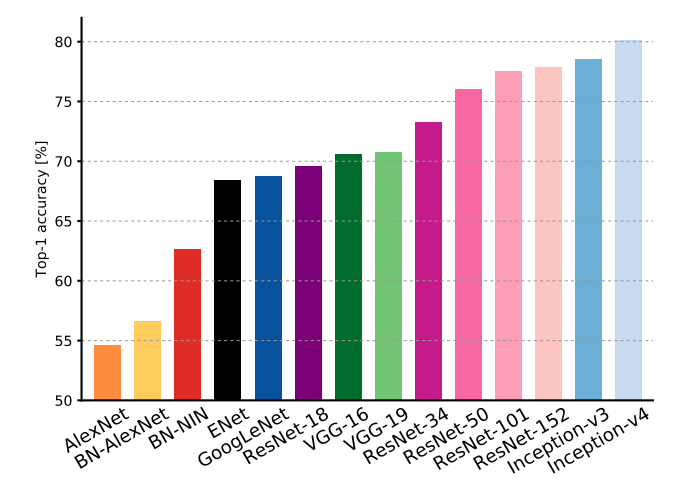
\includegraphics[width=.7\linewidth]{Top1AccuracyOverNetwork.png}
            \caption{Top 1 accuracy vs network. Chart and results from \cite{DeepNeuralNetworkDeployability}}
            \label{Top1AccuracyOverNetwork}
        \end{figure}

        \begin{figure}
            \centering
            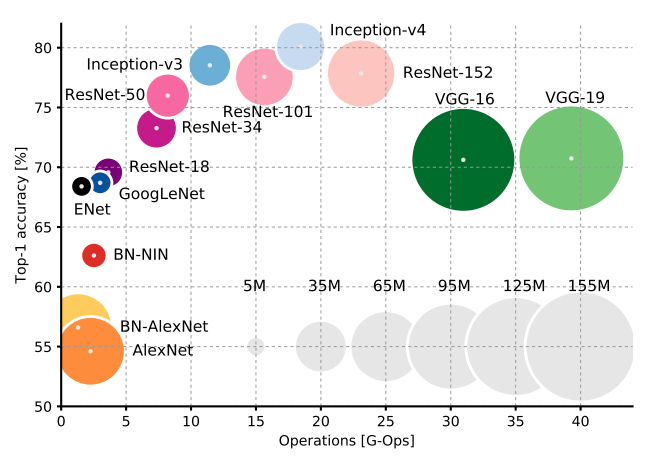
\includegraphics[width=.7\linewidth]{Top1AccuracyOverOperations.png}
            \caption{Top 1 accuracy vs operations, where network size is proportional to parameters. Operations figures are for a single pass (e.g. predicting given a specific input). Chart and results from \cite{DeepNeuralNetworkDeployability}}
            \label{Top1AccuracyOverOperations}
        \end{figure}

        \subsubsection{Datasets}
        %Datasets
        One of the most common datasets, and one of the earliest created, is the NUAA dataset.
        The dataset contains photos of 15 subjects, with faked photos (both flat and warped) being placed in front of the camera.
        Each photo is stored in JPEG format, with a hierarchial structure to show whether the image was real or fake, and what type of
        attack was used (in the case of faked images). One drawback with the NUAA dataset is with regards to licensing: the dataset is only available for
        non-commercial use (i.e. research purposes). This implies that this dataset, and models trained with this dataset, would not themselves be able to be deployed
        \cite{NUAADataset}
        However, as this project is only researching into the feasibility of a web based liveness testing system, this project is for research purposes and hence meeting the
        licensing objectives.

        In 2012, the Replay-Attack dataset was first released, which consists of 1,300 video clips of both photo and video attacks. Each
        set of videos/images are taken under different illumination conditions, and various different attack methods were collected: printed photo, low resolution and high resolution screens with both photos and 
        videos being displayed. The entire dataset consists of several 'subdatasets': the 'devel' dataset is designed as a validation set/training set, while
        the 'test' dataset is designed as a test dataset (and therefore must not be used in the training/validation process). \cite{ReplayAttackDataset}
        % Again, one drawba
            % \todo{Mask Attack Set}

        These two datasets are ideal for testing 2D based liveness systems, since they contain enough samples to reasonable train/test our models. They shall be used
        throughout this project for both training and testing the 2D based liveness models.

        \subsubsection{Temporal-based Liveness Tests}
        These liveness tests require a video input, rather than an image. Rather than looking directly at an image, they mostly look at the differences between the images in a video.
        
        % Blinking
        \paragraph{Blink Detection}
        The blink detection liveness test analyses eye blink behaviour and determines whether the person is real/fake. This liveness test meets our critera for a web-based liveness service,
        as the test doesn't require any extra hardware. Furthermore, a large amount of concious activity from the user isn't necessary, as the video analysed is natural behaviour.
        One drawback of this method is testing: this model requires a video input, which isn't available with the NUAA dataset, and therefore testing this method might be more difficult.
        \cite{BlinkDetectionLivenessTest} Furthermore, this method would be susceptable to a print-based attack where eye holes were cut, since natural eye movement is analysed.
        
        % Face Flashing
        \paragraph{Face Flashing}
        One method, known as the "Face Flashing" liveness detection method, uses the light diffusing off a screen to determine that the input is in fact from the user, rather than from a spoofed recorded/simulated input.
        The method also considers how the light is diffused, as light would diffuse differently based on a face compared to a piece of paper/a screen. \cite{LivenessTestFaceFlashing}
        While this metrics seems very promising at avoiding replay attacks, testing it to a larger degree is more difficult due to the lack of data available for testing, and therefore not implemented for this project.
        One potential drawback though would be with devices that don't have screens but do have cameras, such as with IoT devices. Since a screen isn't present on these, the liveness test wouldn't work. However, for traditional mobile phones/computers
        this would work better.

        Overall, these metrics would be fairly useful on video input, since they take into account the movement/differences between frames, but for implementation purposes they are difficult to test due to lack of datasets available for them
        (since they require special information that isn't available from existing sets). 

        In a web-based approach, the face flashing approach would be particularly useful at determining whether a source-quality image was being fed into the algorithm, since the random face flashing colours would be able to be detected.
        
    \subsection{3D Spoofing Attacks}
        Mask Attacks are a 3D spoofing attack, which involve creating a 3D mask of someone and wearing it. \cite{FaceSpoofingAttacksStudy} These are much less prevalent, but with 3D printing becoming more mainstream, this
        could potentially get more prevalent in the future.

        % Explain the method shown in Choudhary et al., 1999 - SFM. Problem: depth information ahrd to obtain when still with SFM. Noise also problematic.
        % Which uses Structure From Motion.
        In 2013, the 3D Mask Attack Dataset (MAD dataset) was released. This dataset contains 76500 frames of 17 people, recorded using a Kinect camera.
        Each frame contains a depth image, an 2D RGB image with 8 bit colour and a size of 640x480 pixels. Each frame also contains eye positions.
        Real Access samples are contained within the first and second session folders, while the third session contains the frames of mask attacks. The subjects contained
        within each frame are denoted within the filename.
        
        \cite{3DMadDataset}

        \subsubsection{Obtaining 3D data from 2D images/video}
            One method of obtaining 3D data from a video is to use Structure From Motion (SFM). This method was previously utilised in \cite{SFMClassifier} to consider the depth data as a 2D liveness test,
            but this method could potentially work as a solution for obtaining 3D data. However, SFM performs poorly when given a video with a small amount of motion. Furthermore, the 3D mask attack datasets
            available for this project do not contain video but single images, which means such a method would be more difficult to test.

            However, with improved machine learning models, there exist models that can reconstruct facial structure based on a single 2D image. One such model is the VRN model, proposed in \cite{3DReconstructionMethod}.
            The paper, and the associated source code, contains a model that takes a 2D image as input (of size 192x192), and produces a voxel repesentation of the 3D face structure. This model is more suitable for our
            application, since the use of a 2D image rather than a video works well with the datasets available. Furthermore, use of a single 2D image would require less user input as a SFM based method, since the user isn't required
            to move in order to produce an adequate 3D reconstruction. An example of the 3D reconstruction obtained from this model can be seen in Figure \ref{3DReconstructionScreenshot}. The screenshot is obtained from the GitHub repository
            of a Keras-based implementation of this method (since the initial implementation of the paper used the Torch library).

            \begin{figure}
                \centering
                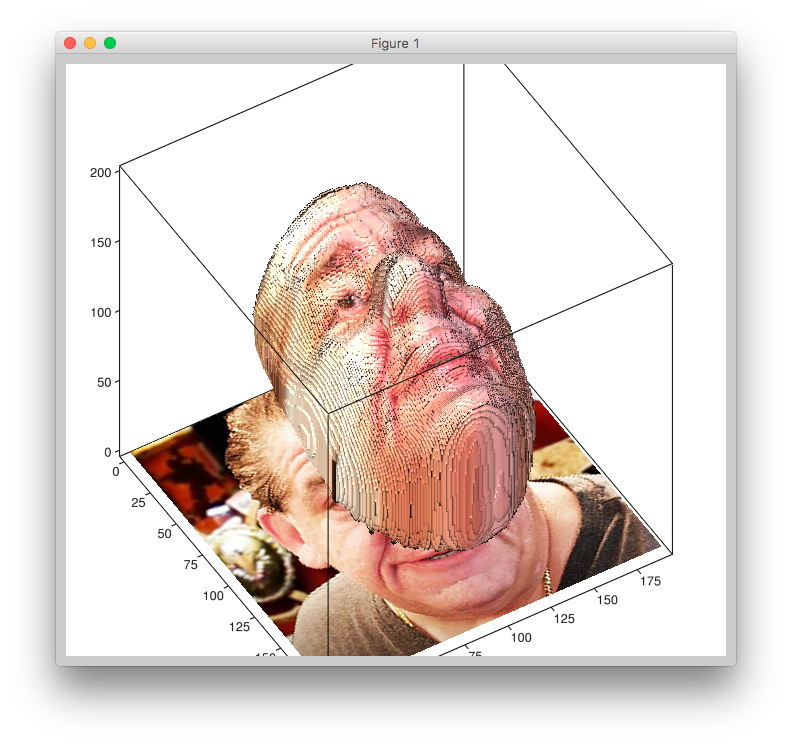
\includegraphics[width=.5\linewidth]{3DReconstructionFromSource}
                \caption{A screenshot from the VRN Torch to Keras version (a conversion of the VRN model to Keras). This screenshot is from \cite{VRNTorchToKeras}}
                \label{3DReconstructionScreenshot}
            \end{figure}

            % \todo{VRN 3D reconstruction on MaskAttackDataset image}

        \subsubsection{3D Classifiers}
            In a similar approach to the 2D methods researched above, there are a variety of existing 3D classifiers that could be repurposed for the liveness classification approach.
            While these methods don't yield the same accuracy figures as with ImageNet, further improvements in the field of 3D classification could lead to better liveness methods in the future.

            \paragraph{PointNet}
                PointNet is a model for classifying point clouds, represented as an unordered set of points. PointNet in total has 3.5 million parameters, with 440 million FLOPs per sample, which 
                is a reasonable number considering other classifiers, but is on the upper end of what would be expected for a web based system. The classifier used within PointNet is a simple feed forward network.
                \cite{PointNet}
                While this model has performance benefits over CNN based models (since 3D convolution is computationally expensive),
                the input is a point cloud structure which might not be the most ideal solution (since sparse data might not be captured, dependent on which reconstruction model is used).

            \paragraph{VoxNet}
                Unlike PointNet, this model uses a voxel representation. This is ideal due to the nature of existing 3D reconstruction models from a 2D image. The accuracy of this classifier isn't the most ideal,
                but improvements could be made such as implementing a Residual network approach (something that worked well for 2D classifiers). As a proof of concept, this model would be ideal to test whether this model would work
                in the real world. \cite{VoxNetModel}
            
\section{Solution}
    % Solution to the problem

    % \todo{Refactor into functional and non functional requirements.}
    A system deployed to the Cloud would require a few important criteria be met. The liveness methods used should be output a liveness score after no more than 2 seconds
    to ensure that such a system doesn't become painful to use by users. The liveness methods should not require any additional hardware (only a normal camera) so that the number
    of devices it can be used by can be maximised. Furthermore, each liveness test must have a reasonable accuracy of over 70\%, to ensure that liveness predictions are fairly reliable.

    The solution built should be focused on the metrics to be used, and fusion of these metrics. While speed is important, network latency and transmission time shouldn't be factored in, 
    since these are incredibly dependent on a client's internet speed/image sizes, and therefore cannot be reliably tested. For small images and reasonably fast internet, latency would be fairly small.

    With these specifications in mind, the design focused on three different liveness tests: an Image Quality assessment based liveness test, a ResNet 50 based classifier (based on a pretrained ImageNet model),
    and a novel 3D based classifer using 3D facial reconstruction models interlinked with the VoxNet 3D classification model. Each of these liveness tests have some common services that are needed; these include
    reading large datasets without causing resource availability problems.

    % \todo{insert diagram of the overall system design (e.g. data, consolidation layer, etc)}

    \subsection{Shared Services}
        \subsubsection{Dataset Managers}
        In order to assess our liveness tests and train them, dataset managers are needed.

        A generic implementation of a dataset was created as an Abstract Class, which was then extended by the NUAA, ReplayAttack and MaskAttack dataset managers.
        This generic implementation allows for future datasets to be easily added, and also provides the class definition of what's needed, to help improve the software engineering process.

        The role of a dataset manager is to load in a dataset from a folder structure (which varies between dataset), conduct any basic preprocessing to convert the files into OpenCV images,
        and produce two H5Py Datasets, one for real images, and one for fake images. The dataset manager also allows further customisation, to load specific subdatasets (such as 'devel' or 'test' in the case
        of the ReplayAttack dataset), or load data regarding specific subjects (in the case of the Mask Attack Dataset). The role of the H5Py dataset is to normalise the datasets into a specific format,
        to allow for easier dataset processing.

        In addition to data normalisation, it also provided a method of reducing RAM usage, therefore allowing larger liveness test models to be created. This is because data is only fetched when needed
        from the hard drive, rather than loading the entire dataset into RAM at once.

        % \todo{Diagram of Dataset management?}

        \subsubsection{Neural Network Infrastructure}
            % Keras to simplify models, tensorflow as the underlying backend.
            % Training machine on Google Cloud, using 64GB RAM, 8 x vCPUs, and an NVIDIA Tesla P100 GPU to improve performance of the training process through parallelism. 
            
            \paragraph{Neural Network Framework} 
            For the 2D and 3D based classifiers, neural networks were to be used. It was decided to use Keras, with the Tensorflow backend, as Keras provides a high level interface to Tensorflow
            and also allows for other backends to be used in the future (which could potentially perform better in different scenarios). The tensorflow backend was used because of the easy configuration
            with both GPUs and without (simply install tensorflow-gpu for GPU processing, and tensorflow for CPU only processing), depending on the machine being used. A high level interface was necessary
            to avoid boilerplate too, since models would be regularly changed to find the best outcome for each classifer.

            \paragraph{Hardware for training}
            Training the neural network required more processing power than was directly available. Google Cloud Compute Engine was used to provide this processing power, since it's easily accessible and has existing
            deep learning environments with Intel-accelerated mathematics libraries. The Google Cloud instance also provided easy extensibility, since some of the liveness tests required additional tools that could not be easily installed
            on NCC/Hamilton clusters at Durham University. Training was conducted on a VM with 64GB RAM, 8 virtual CPUs with an NVIDIA Tesla P100 GPU being used to accelerate the training process (through parallelism).

            \paragraph{Hardware for testing}
            GPUs are expensive, and therefore if such a system were deployed the cost of GPUs would provide expensive to run. Therefore, a CPU only implementation for the testing was followed, using an Intel i7-7700K (at 4.2 GHz), with
            16GB RAM. Performance metrics were yielded using this hardware to emulate the expected performance and understand which metrics performed best and whether they performed adequately.

        \subsubsection{Image Processing and Computation Management}
            OpenCV was used to manage the processing of images, including the image loading components. This library was chosen for the wide support available, and for the large feature set that it provides (including Gaussian Blurring, some image metrics, and some fourier analysis).
            For the rare occasions where OpenCV didn't have the required functionality, scikit-image provided some operations that were necessary.
            
            Numpy was instrumental in most other computation operations (including image preprocessing, mathematical calculations), due to the large speed improvements provided by the C implementation (compared to Python's slower math libraries).
            Since opencv interfaces well with numpy, no conversion was needed which improved the ease of implementation.


        \subsection{Image Quality Assessment Liveness Test}
            \subsubsection{Overview}
            One common way of detecting liveness is to consider the image quality of the camera input. When a printout/screen is held up to the camera, the facial image
            will have some noticable differences, specifically in the high frequencies. There might also be some image compression visible in fake images, compared to real ones.
            This is the basis for this method.

            % \todo{Reference the specification above}.
            More specifically, the implementation was based on the work contained in \cite{ImageQualityAssessmentTest}. 24 different image quality metrics were implemented,
            with metric values being used as an input to a classifier. From previous work, it has been shown that this metric is accurate (therefore detecting spoofing well), while
            also being fairly fast to compute in terms of time, making it ideal for our use-case.

            The classifier being used for our implementation is Linear Discriminant Analysis (LDA).

            A visual explanation of the method can be seen in Figure \ref{ImageQualityLivenessTestDiagram}. 

            \begin{figure}
                \centering
                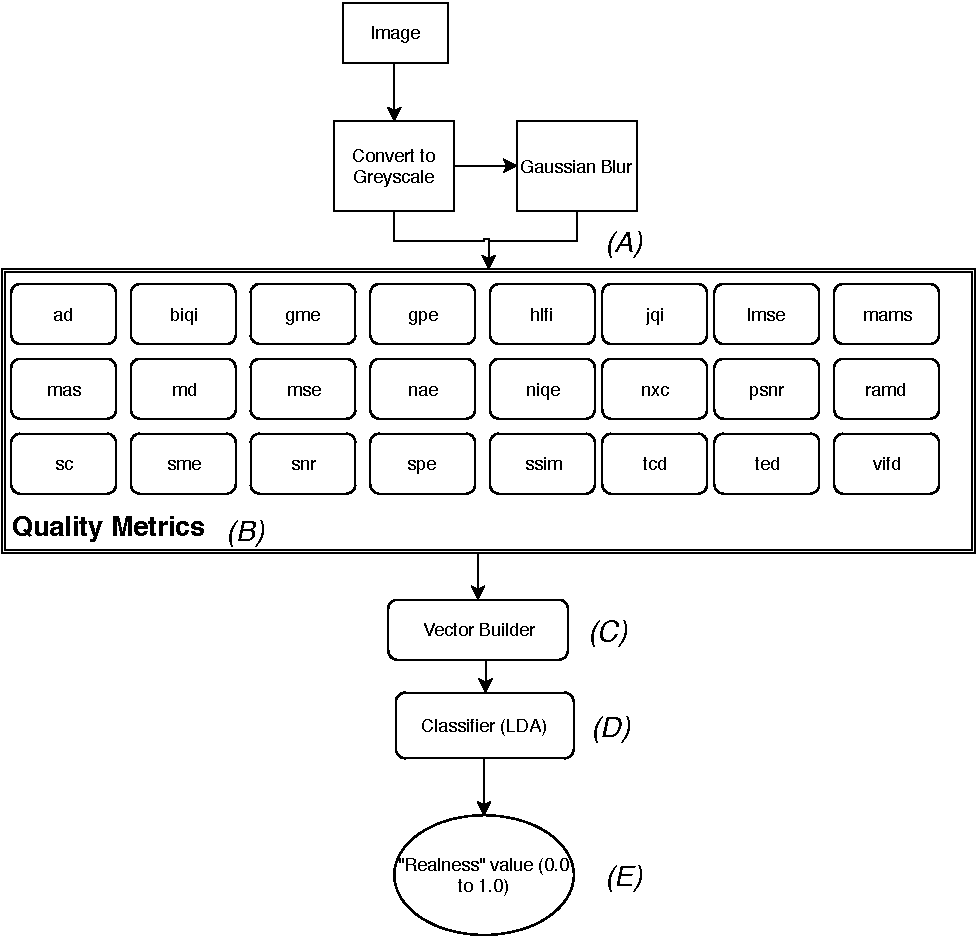
\includegraphics[width=\linewidth]{ImageQualityLivenessTest.pdf}
                \caption{The architecture of the image quality liveness test. (A) The greyscale copy of the image, and a blurred copy of the image are input into each of the metrics.
                (B) The metrics are individually calculated, and a single value output from them. (C) These values build a 1D vector. (D) They are classified using an LDA classifier. (E) The realness value
                is 1.0 for real, and 0.0 for fake, or in between.}
                \label{ImageQualityLivenessTestDiagram}
            \end{figure}
    
            \subsubsection{The Metrics}
            The original paper proposed that 25 metrics were used. However, our implementation used only 24, due to some implementation problems (which shall be detailed below).
                %TODO mention implementation details with RRED.
            There are various different classes of metrics, but each metric is either a full reference metric, or a no reference metric. With a full reference metric, image $I$, and image $I'$ are needed,
            where image $I'$ is the gaussian blur of the original image $I$, with kernel size of $(5,5)$ and $\sigma = 0$. No reference metrics simply require a single image $I$.

            Under the full reference metrics, some methods are based on error sensitivity (image differences, image correlations, image edges, image gradients, and frequency based comparisons),
            structural similarity between the images, or information theoretic based measures.

            Under the no reference metrics, some methods are based on training a classifier (more specifically, a support vector machine), some consider distortion, and the final metric considers the natural scene.
            
            Each of these metrics outputs a single floating point number. These numbers are assembled together into a vector. This vector is then later fed into the next stage (the classifier).

            Most of the error sensitivity metrics were implemented manually using a mixture of Numpy and OpenCV. These were implemented manually based on the implementation guidelines available in the paper.

            For the remaining metrics, some library implementations were used from scikit-image where possible, but in a majority of cases no existing library implementation existed, and as such a new library
            was needed. These methods are outlined below.

            \paragraph{The custom PyVideoQuality library}
            For the SSIM, VIF, and other metrics, no existing implementation existed. Looking back at the original papers for these metrics, a single matlab based implementation existed, which wasn't well documented (due to no comments or
            explanation). This was a problem, since without these metrics it would be difficult to implement this metric.
            
            However, after searching online, a Python 2 implementation was found on GitHub. \cite{VideoQualityOriginal} Therefore, this was forked, and code was converted to Python 3 ready for integration into the project, which included added docstrings to assist the development process. 
            
            In order to allow separation of concerns, it was decided to build a seperate Python package for this. A release on GitHub was created to allow for easy importing from GitHub using pip. The final library implementation can be found on GitHub. \cite{VideoQualityUpdated}


            \paragraph{Blind Image Quality Index Code}
            The Blind Image Quality index implementation followed a similar story to the PyVideoQuality library, as no library implementation existed. A manual implementation was considered, but in order to save time an existing Python 2 implementation was found as a gist \cite{BIQIImplementation}.
            This was converted to Python 3 manually. A manual implementation would have taken more time as this model uses a pretrained classifier, so it would have been required to implement the required preprocessing, train a classifier to an appropriate level,
            and then include this as part of a wider system. Therefore, using this existing implementation seemed the most suitable option due to time available. This implementation required the use of the \emph{pywavelet} library, along with \emph{libsvm} tooling from the command line to train and get the output of the metric.

            % \todo{a big table showing each metric, and implementation details (library vs custom code)}

            \paragraph{The RRED Problem}
            One of the metrics, the Reduced Reference Entropic Distance metric (RRED) was problematic to implement due to the lack of Python implementation available.
            The only implementation available was written in Matlab, and relied on Matlab only libraries. While some had Python equivalents, the steerable pyramid
            functions did not have a Python equivalent, therefore increasing the workload massively for this single metric. Therefore, the metric was ignored for the WIQA
            test, since the test performance without the RRED metric was within the expected range. 
            

            Once these metrics were produced, testing needed to be done to ensure that these metrics were outputting sensible values that could be relied on.
            Two images were selected at random from the NUAA dataset (using the full image path, rather than the dataset manager created beforehand). These metrics
            were then carried out individually on these two images. The values were then compared, to see if they differed, and to detect any potential image quality difference. 
            Testing each of the metrics was slightly challenging as no ground truth data for each metric existed.


        \subsubsection{Classifier}
            Initially, a support vector machine was trialed to test whether a different classifier from the paper \cite{ImageQualityAssessmentTest} would work best. However,
            the performance was fairly unreliable. Adding a grid search to find the optimal parameters still performed fairly pooly, yielding only 70\% accuracy when training and testing on the same dataset. This was poor compared to the expected results from the original paper. Therefore, the classifier was quickly switched to
            use Linear Discriminant Analysis (LDA), which provided far better performance.

            For both classifiers, existing SVM and LDA implementations from the \emph{sklearn} library were used for their performance. 
            
            The default sklearn LDA settings were initially used, but the results produced still weren't ideal. By using an eigenvector based solver, and automatic shrinkage, the LDA model performed far better, yielding the results
            shown in the results section.

            Once a model is trained, it needs to be saved to be used for the testing process. Saving was achieved using the Python \emph{pickle} package. For small models, pickle is ideal since it easily creates a Python object that can be loaded/written
            without additional boilerplate. Since the sklearn classifier models aren't too deep, pickle works. If the models were deeper, then Python's recursion depth limit would hit, causing errors. 
     
            
        \subsection{2D based CNN Liveness Test}
        Recently, 2D convolutional neural networks have had great success in image classification tasks. Systems that use these technologies are currently deployed in real world systems.
        Therefore, by adapting these models to classify facial liveness, it might be possible to obtain a new model, designed for the web (with both low latency and good accuracy).
        
            \subsubsection{Overview}
                As discussed earlier in the paper, there are several different models available for image classification. Unlike imagenet based classifiers, we only have 2 output classes, which are \emph{real} and \emph{fake}.
                Therefore, the final layer of the model would be different, but the remaining details would be identical. Unlike the image quality metric, this metric concerns itself with the facial data, to understand which faces
                are real, and which ones are fake.

            \subsubsection{Data Preprocessing}
                As this metric concerns itself with the facial structure, it became necessary to isolate the face from the input image. Furthermore, as part of the CNN model a required input size was needed to be specified. 
                The preprocessing step therefore needed to produce a facial image that had fixed dimensions.

                This was achieved using the \emph{face\_recongition} package. Using this package, an image is input and a set of bounding boxes is yielded. The largest bounding box (by area) is found,
                yielding the face. Initially, the bounding box was simply cropped and resized to be a square (even if it wasn't initially a square), before being passed to the model. This yielded very poor results,
                due to the difficulty in learning the constantly changing dimensions. As a result, a new method of face isolation based on bounding boxes was designed:

                Given a bounding box $B = (top, bottom, left, right)$, a new bounding box $B'$ which has square dimensions can be created by finding the square
                side width $s$. Mathematically, this is defined as:

                $$s = Max(bottom - top, right - left)$$\\


                Using this, the new bounding box is defined as:


                $$B' = (top, top + s, left, right + s)$$


                By following this method, the model appeared to perform better overall, and produced non-skewed images.

                However, simply isolating the face isn't enough. A fixed size image was needed, in order to be fed into the network. After much experimentation, an image size of $(224, 224)$
                was decided, as smaller dimensions failed to produce adequate results. The resizing was completed using OpenCV.

                
            \subsubsection{The Model}
                    
                \begin{figure}
                    \centering
                    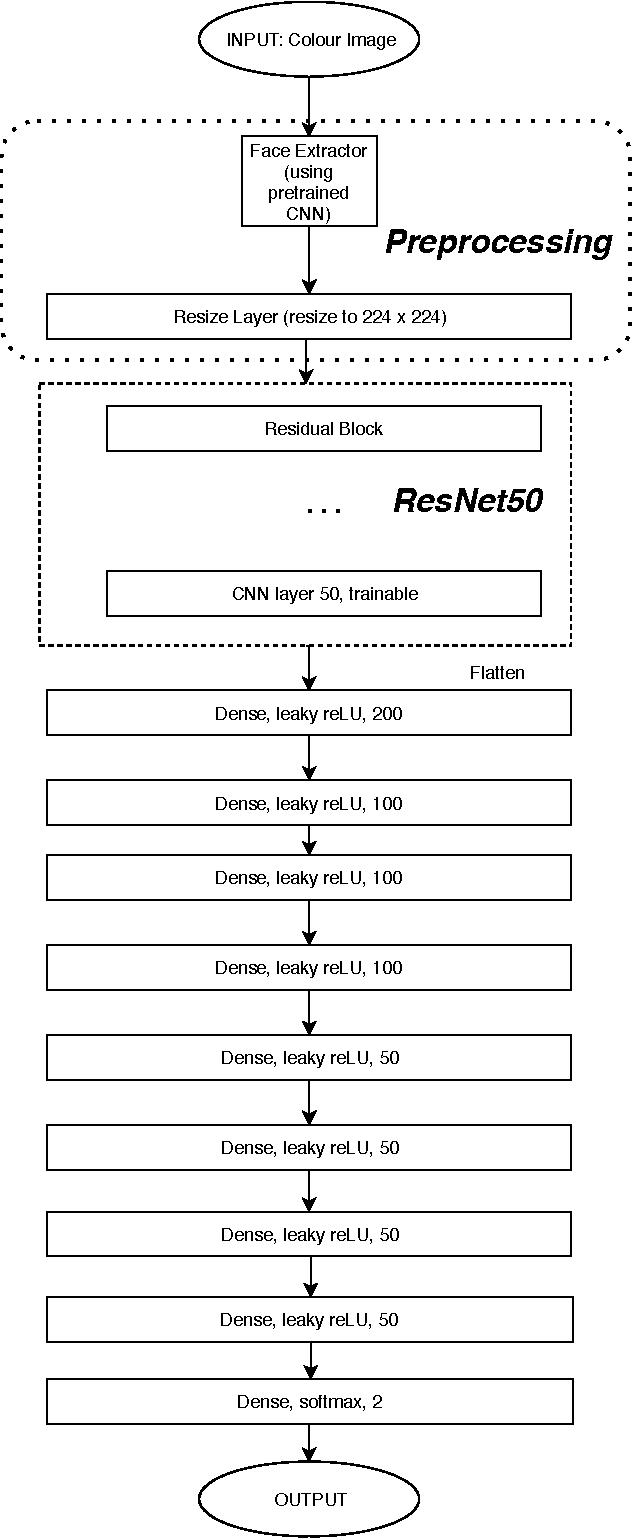
\includegraphics[width=0.5\linewidth]{2DCNNArchitecture.pdf}
                    \caption{The 2D CNN test architecture. We take the face image, resize to a fixed size, and put through ResNet50. The two last CNN layers
                    of this ResNet are trainable. The output of this network is flattened and fed through a deep feed forward network, yielding one output (which is the
                    liveness score as before).}
                    \label{2DCNNArchitecture}
                \end{figure}


                \paragraph{AlexNet}
                Initially, an AlexNet based classifier was designed. While AlexNet performance on the ImageNet dataset isn't as high as other models, it provided an ideal starting point to understand the difficulty
                of the classification. It was eventually found that AlexNet performed relatively poorly on facial liveness classification, and therefore a switch was made to a more complex and better performing model.

                \paragraph{Residual Networks}
                Residual Networks were chosen over VGG and Inception due to their better performance on ImageNet, coupled with their ability to be easily deployed without excessive memory/computation requirements.
                A ResNet 50 architecture was decided upon, as 50 layers seemed reasonable in terms of the available computational power that was available for this proof of concept. It was deemed that if ResNet 50 works, then ResNet 101 might perform equally, if not
                slightly better. A ResNet 50 architecture is an ideal proof of concept.

                While training a model from scratch might have advantages for some applications, a pretrained ResNet50 model from the Keras standard library was used. This was done due to the fairly small amount of data
                available (and therefore using a pretrained model can avoid overfitting), and also to save time learning the basic features that are present in all generic image classification models. Training the entire
                ResNet50 model would require a large number of parameters to be adjusted, so to further reduce the complexity of the training process, only the last layer was set to trainable, with the other layers remaining static.


                \paragraph{Feed Forward Classifier}
                While a CNN is ideal for processing images, a fully convolutional approach to classification didn't seem appropriate. The output from the ResNet 50 model was flattened, and fed directly into a feed forward neural network.
                While pooling layers were considered, these only take the maximum/minimum/average of specific sections, reducing the dimensionality, and the loss of data means the feed forward layer has less information to act upon. Therefore,
                it was instead decided to use no pooling layers. The output from the ResNet is flattened, and fed into an 8 layer feed forward neural network directly. The first layer of this network has a very large number of nodes,
                while the number of nodes is reduced towards the network output.
                
                With the initial experiment, the output layer consisted of a single node, with a sigmoid activation function. The entire network was trained using a binary crossentropy loss function. The network accuracy yielded was fairly reasonable,
                but the confusion matrix showed that the model was outputting \emph{0.0} (fake) for each value, no matter the input. This was a problem, as the network wasn't suitably learning the dataset. As a result, three changes were made to solve the problem, which are outlined below.
                
                \paragraph{The Problem with Activation Functions}
                Initially, the \emph{reLU} activation function was used on all internal nodes within the feed forward network component. While relu is very popular for improved speed over traditional activation functions such as tanh and sigmoid,
                for negative values it has a problem. ReLU is positive for all positive values, but 0 for all negative values.

                While all inputs were non-negative, weights could lead to these values becoming negative. There is a known problem called "dying ReLU", where some neurons output 0
                due to having a negative input (the weights and inputs for all input neurons sum to a non-positive value). Therefore, the model was able to learn 0 (fake) easily, but
                couldn't learn real (1.0) at all. \cite{liu_liu_2017}

                This problem was counteracted by changing activation function from reLU to Leaky ReLU. Unlike reLU, leaky relu isn't zero when negative. It requires an input value $\alpha$, which is used
                as the gradient of the line when less than zero. \cite{liu_liu_2017} For this model, $\alpha=0.3$. The activation function is defined formally as:
                
                \begin{equation}
                    Activation(x) =
                    \begin{cases}
                    x, & \text{if}\ x>0 \\
                    \alpha \cdot x, & \text{otherwise}
                    \end{cases}
                \end{equation}

                \paragraph{The Problem with a Single Neuron Output}
                In order to mitigate the problem of outputting all zeros, the output method of the network was changed. Instead of a single neuron, giving a realness value, two neurones were used.
                These neurons would use the softmax activation function, rather than the sigmoid activation function, to ensure the sum of the neuron outputs would be zero (therefore giving a probability that can be used).
                The use of two neurons to encode the realness means that the nature for a network to learn 0 is slightly removed, as there will always be a non-zero output for one of the neurons expected. The encoding method used here
                is called one-hot encoding in the literature.

                \paragraph{Normalization and Dropout}
                Batch Normalization and dropout were both used within the feed forward network component to improve learning and reduce the risk of overfitting. Overfitting was a concern due to the small dataset that was used for training.
                Batch Normalization layers were added between each dense layer, which resulted in increased accuracy of the model.



                Throughout the experimentation process, the model was found to be overfitting. Therefore dropout was added (with a dropout level of 0.3) between each dense layer. This reduced the effects of overfitting.

                The overall outcome is shown in Figure \ref{2DCNNArchitecture}. The normalization and dropout are not visible in the diagram, since they are only used for training.


            \subsubsection{The Training Process}
                \paragraph{Optimizer}
                Initially, the Standard Gradient Descent was used as the optimizer. This was chosen due to the findings of \cite{SGDBetterThanAdamForImageClassification},
                which advised that SGD was better than the Adam optimiser for producing models that generalise. However, after experimenting further the Adam optimiser appeared
                to generalise better for this project. Using the SGD optimizer, the validation accuracy fluctuated with fairly poor accuracy results overall. The Adam optimizer
                didn't fluctuate, and the accuracy yielded was much higher.

                It's possible that SGD might perform better over longer periods of time with a very small learning rate, but due to time constraints and the need to experiment and show a proof of concept,
                Adam proved better for the purposes of this project.


                \paragraph{Loss Function}
                    Initially, while the model had a single neuron output, the binary cross entropy loss function was used as it's suitable for a single binary output.
                    However, when the two neuron output model was introduced, the loss function was changed to use categorical cross entropy as this was the most suitable
                    for a categorical one hot encoding method.

                \paragraph{Data Generators}
                    Due to the large amount of data being processed, it was necessary to use a data generator to conduct the preprocessing on the fly. While the preprocessing
                    could have been saved to disc, the preprocessing steps were changed throughout the project, therefore defeating the benefits of such an optimisation.

                    Initially, Keras' built-in ImageDataGenerator was used, as it allowed for a preprocess function to be passed in. While this works for a preprocess function that yields the same shape image
                    as was input, Keras' ImageDataGenerator does not support resizing images within the preprocess function (e.g. for cropping).

                    Initially, a Lambda expression within the network was used to resize the image, but this led to problems with saving/loading models (due to Tensorflow being necessary).
                    Therefore, a custom data generator was written from scratch. With this new generator, it wasn't necessary to follow this size constraint within the preprocess function.


    \subsection{3D Face Reconstruction Liveness Test}
        \subsubsection{Overview}
            While 2D methods work well for traditional paper/screen based attacks, they are not designed for detecting the wearing of 3D masks. With 3D printing
            becoming more common, and automatic mask generators also becoming available online, this type of attack is becoming more common.

            The method proposed merged recent developments in facial reconstruction with recent deep learning models for classifying 3D data, to investigate a proposed
            architecture for a 3D classifier. Unlike previous methods, face data is captured in 2D using a standard device camera, before being reconstructed and then classified.

        \subsubsection{2D Image Preprocessing}
            The 2D preprocessing step followed a similar process to the previous liveness test proposed. A CNN based face detector produced a set of bounding boxes, and a square face image was produced
            following the same method as was proposed previously. Unlike the previous method, the image was resized to a fixed size of (192, 192) in colour. This size was necessary due to the requirements
            of the pretrained model.

        \subsubsection{3D Facial Reconstruction}
            A method of obtaining facial structure from a 2D image was required. While video based methods such as Structure From Motion exist, they require a video input which has a large variety in motion, which might not be available/obtainable.
            However, recent research has developed a method known as VRN, which is a neural network designed to produce 3D facial structure from a single 2D image. \cite{3DReconstructionMethod}
            While the original work was built using the Torch deep learning framework, a pretrained model with appropriate source code exists for Keras. \cite{VRNTorchToKeras} This pretrained model
            takes an image of size (192, 192) in, and produces a 3D voxel based representation. 

            In order to correcly modularize the system, the \emph{FaceVoxelBuilder} class was produced to correctly load the pretrained model, and build the voxel structure for either 1 image, or multiple images (in the case of batch training).

            While implementing this component of the system, there was a problem: Tensorflow didn't build the objects from the pretrained model correctly in some cases, as certain components of the model didn't exist on the graph. This was solved by manually creating the predict function by calling a private helper function (\emph{model.\_make\_predict\_function()}).
            This was a known issue with the version of Keras that was being used, and the solution found was specified by the developers of the framework. \cite{KerasVoxNetBug}

        \subsubsection{3D Classification}
            While 2D image based classifiers exist, and perform well, this isn't the case with 3D image classifiers. A VoxNet based classifier was chosen due to the adequate performance on the SUOD dataset (of 69\%),
            coupled with the relatively small model size. \cite{VoxNetModel} While this model can in future be improved and adjusted, this classifier was believed to produce results that could show a proof of concept,
            and determine whether this method would be suitable for a web-based liveness system. The final architecture is shown in Figure \ref{3DClassifierArchitectureDiagram}.

            \begin{figure}
                \centering
                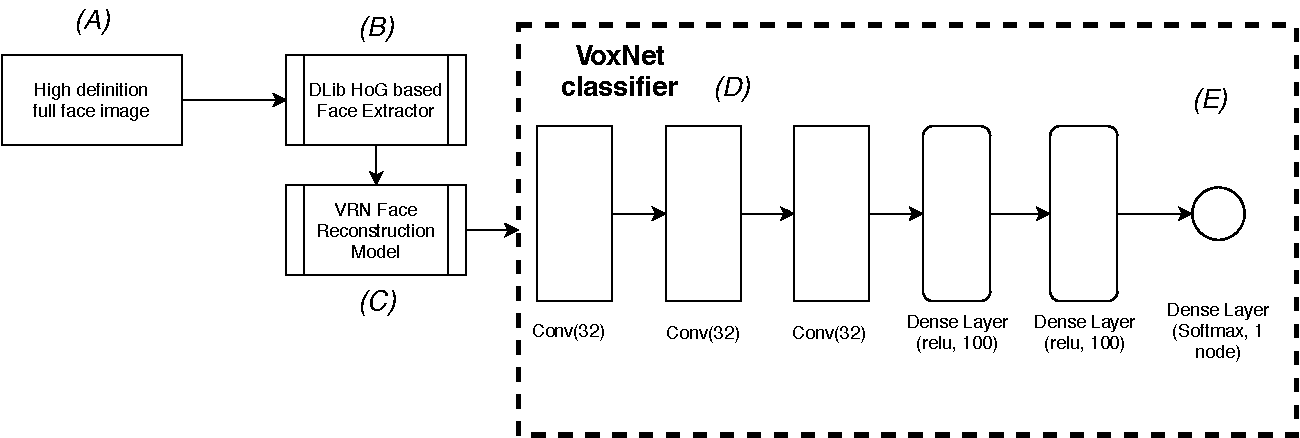
\includegraphics[width=\linewidth]{voxnet.pdf}
                \caption{
                    This is an overview of the 3D classifier. \textbf{(A)} a high resolution image is input into the classifier. \textbf{(B)} The image goes through a HoG based face detector. The bounding box of the face is extracted, and the image is cropped. 
                    The image is then resized to be 192x192 pixels, which is what's required by the VRN process.
                    \textbf{(C)} The pretrained VRN face reconstruction model takes an image input, and outputs a voxel representation. Some postprocessing from the VRN model 
                    is necessary to convert an occupancy grid into a voxel representation (this is done here rather than in the VoxNet model).
                    \textbf{(D)} The VoxNet classifier uses several 3D convolutional layers, along with a couple of Dense layers to classify.
                    \textbf{(E)} The output of the last dense layer is simply a single number defined as the certainty of realness. 1.0 implies the model is certain that the input is real, while 0.0 implies the model is certain that the input is faked.
                }
                \label{3DClassifierArchitectureDiagram}
            \end{figure}

        \subsubsection{The Training Process}
            Training was conducted using a binary crossentropy loss function, with an Adam based optimizer. Binary cross entropy was used since there was only a single output node,
            compared with a categorical approach. 

            In order to conduct training, a Data Generator was used to minimize memory constraints, since the entire dataset didn't need to be loaded into memory after being preprocessed. Instead,
            only a single batch would be preprocessed on the fly, thus reducing memory usage considerably.

            While training, a problem with the built in data generators was encountered. While 2D images were being input, a 3D representation was required as output from the data generator,
            something that the Keras ImageDataGenerator wasn't able to deal with. Initially, the VRN model was included as part of the classification model. This would see a 2D image being input into the model,
            and the model would reconstruct to 3D and classify all in the same model. While this is a more monolithic approach, it would avoid the need to switch out the ImageDataGenerator. However,
            when implemented this didn't work: the 3D reconstruction process required non-tensor operations (more specifically, the use of the stack command), which could not be included as a network layer.

            Therefore, the final solution was to instead conduct the 3D reconstruction as a preprocessing step, and led to the replacement of the Keras ImageDataGenerator with a custom generator, designed to output 3D from 2D input.
            This custom generator would resize the images, reconstruct the 3D representation, and return the appropriate batch yielded. This solved the problem.

        \subsubsection{The Dataset}
            Unlike the previous two liveness tests, this liveness test relied on a completely different dataset, the Mask Attack Dataset (MAD). \cite{3DMadDataset}
            The goal of this liveness test was to detect mask based attacks (and more widely, 3D based attacks), and this dataset was used due to it being more repesentative of the problem
            than the ReplayAttack and NUAA datasets (which are designed for 2D based attacks).

            Unlike the 2D based methods, two datasets weren't used in a cross validation style assessment of the method, so instead the MAD dataset was split by subject (the person being spoofed):
            half of the subjects were used for the training/validation sets, and the other half were left for training purposes.

            Subjects 1,2,3,4,5,6,7 were used for training purposes, and 8,9,10,11,12, 13 were used for testing purposes. Splitting up the dataset in this way was necessary to correctly assess the classifier,
            to ensure results give a true indication of how well the model learned the features, rather than how well the model learned the dataset.

  
\section{Results}
    % based on the solution, what results did we yield? What did we find out?
    For both liveness tests, cross dataset validation/testing was conducted. Each model was trained using the entire NUAA dataset, and the Replay-Attack test set
    was used to measure the results shown below. In the case of the 2D Convolutional Neural Network (CNN), a validation set was required to ensure the model performed
    well, so in this case the Replay-Attack devel set was used. It must be noted that no overlap occurs between the Replay-Attack devel and test sets, to prevent the risk
    of these results being invalid.

    \begin{table}[ht]
        \centering
        \begin{tabular}[t]{lcc}
            \toprule
             & \textbf{Image Quality Liveness Test} & \textbf{2D CNN Liveness Test}\\
             \midrule
            \textbf{Accuracy (\%)} & 87.0 & 71.2\\
            \midrule
            \textbf{True Negatives (\%)} & 37.5 & 71.5\\
            \textbf{False Positives (\%)} & 12.5 & 1.37\\
            \textbf{False Negatives (\%)} & 0.5 & 22.5\\
            \textbf{True Positives (\%)} & 49.5 & 4.69\\
            \bottomrule
        \end{tabular}
        \caption{Table of results, showing test accuracy with the percentage of test results falling into the specific category defined in the confusion matrix (obtained using sklearn).}
        \label{ResultsTable}
    \end{table}

    \begin{table}[ht]
        \centering
        \begin{tabular}[t]{lcc}
            \toprule
             & \textbf{Image Quality Liveness Test} & \textbf{2D CNN Liveness Test}\\
             \midrule
            \textbf{Time to load (s)} & 0.00104 & 7.44\\
            \textbf{Time to classify 1 image (s)} & 1.40 & 1.04\\
            \bottomrule
        \end{tabular}
        \caption{Table of results, showing the wall clock time for the load and predict phases of both liveness tests.}
        \label{WallClockResultsTime}
    \end{table}
    % CNN table: 4317 & 83 & 1357 & 283
    \subsection{Image Quality Liveness Test}
        Overall, the Image Quality Test performed as expected with reference to the initial paper. Unlike the original paper however, instead of isolating the face
        from the input image, the entire image was used. While isolating the face might perform well, using the entire image might provide further subtle information
        about the image quality.

        The overall results, shown in Table \ref{ResultsTable} show fairly good performace on the ReplayAttack test dataset, with an accuracy of 87\%. This is in line with
        what was expected from the paper \cite{ImageQualityAssessmentTest}. While accuracy gives an overall account of the results, it doesn't show the overall performance.
        
        The level of true negatives and true positives respectively are fairly high, but the number of false positives was slightly higher than expected (i.e. where the model predicts someone to be real where they are actually not).
        What's interesting to note is the low number of false negatives (indicating someone is fake where they are real), which in our security concious case isn't wanted (since inconvenience isn't as much of a problem as security).
        However, the overall performance was better than expected.
        % Total results - the RAW data in case people need it.
        % 0.87
        % True Negatives:  75
        % False Positives:  25
        % False Negatives:  1
        % True Positives:  99
        While accuracy is important, the time taken for the model to classify a single image is also important. The LDA method took 1.40 seconds to classify a single 2D image, which is within the specified 2 seconds bound.
        Also, the model itself is very small and therefore can be loaded in a very minute amount of time (0.001 seconds). The bulk of the time required is in the calculation of the metrics, rather than the classification process,
        and therefore future speed optimisations could consider optimising the calculation of the metrics. These results can be seen in Table \ref{WallClockResultsTime}.

    \subsection{2D Convolutional Neural Network Liveness Test}



        The overall performance of our liveness test can be seen in Table \ref{ResultsTable}. While not as accurate as the previous model, the model still detects true negatives with a fairly high percentage.
        While the overall accuracy of this model could be improved with further training or by deepening, the results show that this basic architecture is feasible. In the security conscious environment of facial liveness,
        false negatives, while potentially annoying to the end user, are an ideal result compared to false positives (which would imply that someone is real when they are fake). While false positives still exist, their number is small compared to the number of negatives.
        Furthermore, the number of positives is small, meaning that this model leans on the side of caution, something that is ideal. Therefore, this model would be secure and accurate enough with further training (and potentially replacing ResNet50 with a deeper ResNet model).

        The time taken to load the model from memory was the main bottleneck in terms of computational performance, as loading the model into memory for the first time took 7.44 seconds. However, once the model was loaded,
        the time taken to predict a single image is very small, on average taking 1.04 seconds, which is even smaller than the W-IQA test, and almost half the specified 2 second time, which is ideal. These results can be seen in Table \ref{WallClockResultsTime}.     
        % Confusion Matrix = [[4317  283]
%           [1357   83]]

    
    \subsection{3D VoxNet Liveness Test}
        This method had some major performance challenges. The 3D facial reconstruction worked well, producing the desired outcome. However, the 3D classifier (VoxNet), had numerous problems.
        The original VoxNet model, proposed in \cite{VoxNetModel}, used 32 filters for the Conv3D layers (with a 32x32x32 input). However, using 32 filters in our model for each Convolutional Layer (alongside the larger data input than expected),
        led to memory errors and wasn't able to be trained on the training hardware.  Reducing the 3D reconstruction resolution wasn't an option, since the entire model would require retraining (which would take lots of time, resources, and wasn't feasible).
        Furthermore, as seen with the 2D CNN method, reducing the resolution might also reduce the accuracy. Therefore, the remaining solution was to reduce the number of filters down to a small 12 filters per convolution layer.

        During the training process, with a variety of learning rates, the accuracy of the model didn't leave 50\% with a differing amount of batch sizes. This indicates that the model wasn't learning the features correctly (potentially due to the lack of filters in the Convolutional Layer).
        
        While the classifier itself didn't work and yield any meaningful results, it's also important to consider the time taken for a 2D image to be reconstructed. 
        To reconstruct a single image from 2D to a 3D face structure, it took 5.39 seconds, which already exceeds the 2 second constraint set by the specification.

        Due to the poor accuracy with a low number of filters, the excessive amount of memory required for unknown accuracy results, and the large time taken to reconstruct the 3D structure (not including the added time to theoretically classify the result),
        this liveness test clearly isn't feasible for the purpose of a web liveness service.

\section{Evaluation}
    % How well our system works, how well did it assess stuff, and how it can be improved.
    % what are the uses of our research? e.g. influence and improve the design of xyz...
    \subsection{Usefulness of our system}
    
        % Identified two metrics that could be deployed.
        % Created the structure of such a system (e.g. consolidation layer) to allow for future extensions with further liveness tests.
        % Applications: within IoT devices, use within web browsers alongside existing face recognition services. 
        % There is an argument that one could steal your likeness and use it elsewhere on the internet. However, providing liveness tests
        % are suitable, there is no other way of stealing ones face. There would be a need to ensure furhter development of such a system.
        % Developing a single component as a service would mean developers could focus on developing their applications. 
        \paragraph{Quality Test}
            The Quality Test performed well, and is suitable for a web based liveness service due to the high 87\% accuracy achieved.
            True positives and true negatives (that is, correct predictions for both real and fake) were high which means that the classifier
            is classifying correctly. However, the high false positive rate shows a slight cause for concern, since the model in 12.5\% of cases
            classified a fake image as real, which isn't ideal for our security focused solution. This could potentially be solved by adjusting output
            variable of the classifier (using a figure representing 'fakeness' rather than realness). This would hopefully lead to more false negatives,
            which are inconvenient but more secure for the system.

            In terms of computational performance, a 1.40 second time for classifying a single image is within the limits of the expected 2 seconds, and could be improved further
            with parallel based methods, and not relying on libsvm for the BIQI metric.
        \paragraph{2D CNN}
            The 2D CNN Test performed adequately. While the accuracy was lower than expected (at 71\%), the classifier itself still performed better than random.
            Furthermore, the model was very good at classifying true negatives, with a total percentage of 71.5\% being true negatives. While the model itself had
            a higher than expected false negative percentage, this is just inconvenient for the user rather than a security problem. The model showed it could classify true
            positives, but this figure was fairly low. This could be improved by improving the training process: ensuring each input image has a correctly identified face (as
            some images without a detectable face would have been left to classify the entire image, just resized to the input size). The less noise in the input data, the better the potential
            results in the future. Furthermore, using a larger ResNet model, such as ResNet-101 could lead to better results.

            In terms of performance, classifying an image is very quick, but the time taken to load the model is what took the most time (due to memory needing to be allocated and written to).
            In production, providing a model was preloaded and ready to accept input, the computation time of this metric would be very fast, and therefore be ideal for inclusion in a liveness web service.
        \paragraph{3D VoxNet Liveness Test}
            As seen from the results, this method of liveness test isn't feasible. With extra training, while the accuracy of the model could be improved, the
            real time memory requirements don't seem feasible. Based on the VoxNet paper, the accuracy achieved with a 32x32 VoxNet classifier on the SUOD dataset (a 3D dataset of objects)
            is 69\%. While this accuracy could be justified with reasonable computational and memory characteristics, this further proves that this method isn't feasible in the current state. In the future, a new approach of detecting 3D attacks is necessary.
    \subsection{Improvements}
        \paragraph{Representing 3D Attacks}
        While our system works fairly well for 2D based attacks, performance for 3D based attacks definitely needs work.
        While our VoxNet based method didn't yield any meaningful results, there is a chance that a 2D image could yield results
        with 3D based attacks (using a residual network on a static image to detect minor mask-based imperfections), or alternatively
        considering a sequence of images using LSTMs to detect changes in movement. This however would require video input, meaning the
        NUAA dataset wouldn't be useful.

        \paragraph{Preventing Source-Quality Web Browser Attacks}
        Current approaches followed (including ones in this paper) assume that the video capture and liveness processing is conducted securely, 
        without any interference from malicious actors. However, in the case of web browsers, the video capture process might not be secure as
        the client-side code can be easily tampered with, and therefore shouldn't be trusted fully. The solution to this is a random video input,
        something requested by the server and required to be contained within the video (similar to a CSRF token in web forms). The answer to this
        is contained within an existing liveness metric: a motion based one. The process of face flashing would be ideal, as a specific colour could
        be requested, and expected to be visible in the frame. Alternatively, head tracking and expecting a specific set of motions would also be suitable,
        but as this would require user input might not be favourable.

        % TODO might be a way of explaining tampering with getusermedia.
        
        \paragraph{Existing BIQI implementation}
        Currently, the BIQI implementation requires the use of a subprocess to call libsvm based commands on the system. Instead of using standard output, files are used which
        cause a reduction in speed.
        Speed isn't the only problem here, as scaling would become a problem due to the existing implementation. 

        To fix this problem, a reader would be needed to import a trained libsvm model into sklearn, and the code would then need to be refactored to use the updated sklearn model. 

        \paragraph{Privacy/Legal Considerations}
            While the security of a facial liveness cloud service is reasonable, there would be some legal concerns to consider in the deployment of an actual application.
            Face data, as with all biometric data, is classed as sensitive personal data. This can be found in the GDPR definitions, from \cite{GDPRDefinitions}. As such, care would need to be taken in the development of such a system
            to ensure compliance. While the details below are not legal advice, these would be the starting point to building a liveness service that's more compliant.

            % Source: https://thenextweb.com/contributors/2018/10/29/heres-how-face-recognition-tech-can-be-gdpr-compliant/
            When designing such a service, collecting user consent is necessary through a positive opt-in (without any prefilled tick boxes). In addition to collecting consent, users must be able to withdraw their consent too.
            Naming any third parties might be necessary too, especially if using a Cloud-based service. Furthermore, some anonymisation process would need to be implemented to ensure that the image isn't easily identifiable (therefore names
            must not be recorded). Therefore, no user accounts of persistent storage tieing people to their faces would be ideal, to ensure anonymisation. While a facial liveness web system would be securing a facial recongition system, the 
            liveness system itself would need to be secure in order to meet GDPR regulations. \cite{GDPRForFacialRecognition} Encrypting data in transit is fairly easy, using SSL is a modern standard
            and certain browsers require the use of SSL for accessing certain media APIs. Encryption of data at rest might be necessary, but since the image wouldn't necessarily be stored that might not be required. 
            

            Aside from GDPR, licensing of datasets is another concern. The Replay-Attack dataset is licensed on condition of research, rather than for commercial use. 
            As such, the deployed version of such a liveness based system would need to use a network trained with a new dataset that has the appropriate licensing (either a bespoke one, or one that is public domain).

\section{Conclusions}
    % overall, what did the project show?
    % TODO this needs to probably be reworded.
    This project showed that creating a facial liveness service for the web is a feasible idea, and performs fairly well for 2D attacks, with adequate accuracy and computational requirements.
    The image quality liveness test is accurate and fast, while the ResNet based method is a feasible idea and performs adequately, and could be improved further to improve the accuracy. For 3D attacks however, the
    proposed VoxNet based model performed badly and is not recommended for inclusion in a liveness test web service.

    In addition, the improvements to the existing system were shown, and potential GDPR considerations were shown on how to implement such a system to better comply with the regulation. In building of a system for commercial use, it's important
    to note that licensing on training and testing datasets would require new datasets be used.

\printglossary
\bibliographystyle{abbrv}
\bibliography{report}

\end{document}